%%%%%%%%%%%%%%%%%%%%%%%%%%%%%%%%%%%%%%%%%%%%%%%%%%%%%%%%%%%%
%%  Class 35, NE 155
%%

\documentclass[xcolor=x11names,compress]{beamer}

\definecolor{CoolBlack}{rgb}{0.0, 0.18, 0.39}
%% General document %%%%%%%%%%%%%%%%%%%%%%%%%%%%%%%%%%
\usepackage{graphicx}
\usepackage{tikz}
\usetikzlibrary{decorations.fractals}
\usepackage{hyperref}
%%%%%%%%%%%%%%%%%%%%%%%%%%%%%%%%%%%%%%%%%%%%%%%%%%%%%%

%% Beamer Layout %%%%%%%%%%%%%%%%%%%%%%%%%%%%%%%%%%
\useoutertheme[subsection=false,shadow]{miniframes}
\useinnertheme{default}
\usefonttheme{serif}
\usepackage{palatino}
\usepackage{tabu}
\usepackage[normalem]{ulem}
% Links
\usepackage{hyperref}
\definecolor{links}{HTML}{003262}
\hypersetup{colorlinks,linkcolor=,urlcolor=links}

% addition of color
\usepackage{xcolor}
\definecolor{CoolBlack}{rgb}{0.0, 0.18, 0.39}
\definecolor{byellow}{rgb}{0.55037, 0.38821, 0.06142}
\definecolor{dgreen}{rgb}{0.,0.6,0.}
\definecolor{RawSienna}{cmyk}{0,0.72,1,0.45}
\definecolor{forestgreen(web)}{rgb}{0.13, 0.55, 0.13}
\definecolor{cardinal}{rgb}{0.77, 0.12, 0.23}

\setbeamerfont{title like}{shape=\scshape}
\setbeamerfont{frametitle}{shape=\scshape}

\setbeamercolor*{lower separation line head}{bg=CoolBlack}
\setbeamercolor*{normal text}{fg=black,bg=white}
\setbeamercolor*{alerted text}{fg=dgreen} % just testing; I think this looks better
\setbeamercolor*{example text}{fg=black}
\setbeamercolor*{structure}{fg=black}

\setbeamercolor*{palette tertiary}{fg=black,bg=black!10}
\setbeamercolor*{palette quaternary}{fg=black,bg=black!10}

% Margins
\usepackage{changepage}

\mode<presentation>
{
  \definecolor{berkeleyblue}{HTML}{003262}
  \definecolor{berkeleygold}{HTML}{FDB515}
  \usetheme{Boadilla}      % or try Darmstadt, Madrid, Warsaw, Boadilla...
  %\usecolortheme{dove} % or try albatross, beaver, crane, ...
  \setbeamercolor{structure}{fg=berkeleyblue,bg=berkeleygold}
  \setbeamercolor{palette primary}{bg=berkeleyblue,fg=white} % changed this
  \setbeamercolor{palette secondary}{fg=berkeleyblue,bg=berkeleygold} % changed this
  \setbeamercolor{palette tertiary}{bg=berkeleyblue,fg=white} % changed this
  \usefonttheme{structurebold}  % or try serif, structurebold, ...
  \useinnertheme{circles}
  \setbeamertemplate{navigation symbols}{}
  \setbeamertemplate{caption}[numbered]
  \usebackgroundtemplate{}
}
%---

\renewcommand{\(}{\begin{columns}}
\renewcommand{\)}{\end{columns}}
\newcommand{\<}[1]{\begin{column}{#1}}
\renewcommand{\>}{\end{column}}

% adding slide numbers
\addtobeamertemplate{navigation symbols}{}{%
    \usebeamerfont{footline}%
    \usebeamercolor[fg]{footline}%
    \hspace{1em}%
    \insertframenumber/\inserttotalframenumber
}

% equation stuff
\newcommand{\Macro}{\ensuremath{\Sigma}}
\newcommand{\Sn}{\ensuremath{S_N} }
\newcommand{\vOmega}{\ensuremath{\hat{\Omega}}}
\usepackage{mathrsfs}
\usepackage[mathcal]{euscript}
\usepackage{amssymb}
\usepackage{amsthm}
\usepackage{epsfig}
\usepackage{amsmath}
%%%%%%%%%%%%%%%%%%%%%%%%%%%%%%%%%%%%%%%%%%%%%%%%%%
% title stuff for footer
\title{NE 155}
\author{R.\ N.\ Slaybaugh \\
(well, Max Fratoni!)}
\date{April 20, 2015}

\begin{document}

%%%%%%%%%%%%%%%%%%%%%%%%%%%%%%%%%%%%%%%%%%%%%%%%%%%%%%
%%%%%%%%%%%%%%%%%%%%%%%%%%%%%%%%%%%%%%%%%%%%%%%%%%%%%%
\begin{frame}
\title{NE 155\\Introduction to Numerical Simulations in Radiation Transport}
\subtitle{Lecture 34: Geometry and Collisions}
\titlepage
\end{frame}


%%%%%%%%%%%%%%%%%%%%%%%%%%%%%%%%%%%%%%%%%%%%%%%%%%%%%%
%%%%%%%%%%%%%%%%%%%%%%%%%%%%%%%%%%%%%%%%%%%%%%%%%%%%%%
\begin{frame}{Outline}

    \begin{enumerate}
    \item Overview of Monte Carlo for Neutron Transport
    \item Basic tracking of particles through a geometry
      \begin{itemize}
      \item Determining next event location
%Sampling flight path
%Distance to boundary in analytic
%geometry
      \item Next event selection
      \item Next event processing
      \end{itemize}
    \item Collision Physics
      \begin{itemize}
      \item Sampling target nuclide
      \item Sampling reaction type
      \item Sampling exit energy
      \item Sampling exit direction
      \item Sampling exiting particles
      \end{itemize}
    \end{enumerate}

\vspace*{1em}
Notes derived from Jasmina Vujic and Paul Wilson
\end{frame}



%%%%%%%%%%%%%%%%%%%%%%%%%%%%%%%%%%%%%%%%%%%%%%%%%%%%%%
%%%%%%%%%%%%%%%%%%%%%%%%%%%%%%%%%%%%%%%%%%%%%%%%%%%%%%
\begin{frame}{Learning Objectives}

    \begin{enumerate}
    \item Be able to provide MC transport algorithm
    \item Understand basic tracking of particles through a geometry
      \begin{itemize}
      \item Understand the steps necessary for tracking particles
      \item Understand the use of mean free path
      \item Sample the distance to the next physics event
      \item Compute the distance between a point and surface along a given direction
      \item Determine next event
      \item Process outcome of next event
      \end{itemize}
    \item Understand ...
    \end{enumerate}

\end{frame}


%%%%%%%%%%%%%%%%%%%%%%%%%%%%%%%%%%%%%%%%%%%%%%%%%%%%%%
%%%%%%%%%%%%%%%%%%%%%%%%%%%%%%%%%%%%%%%%%%%%%%%%%%%%%%
\begin{frame}{Monte Carlo for Transport}

  	\begin{figure}
  	\begin{center}
  		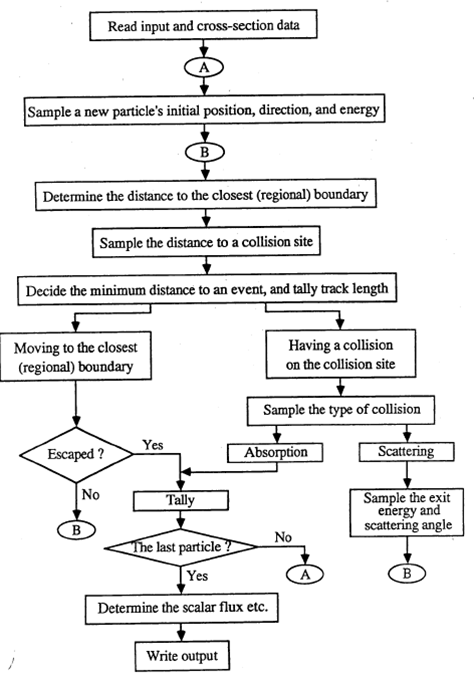
\includegraphics[height=3in,clip]{MC-algorithm}
	\end{center}
  	\end{figure}
  	% we've covered some of the basics that surround this algorithm,
  	% today we'll start covering some of the nuts and bolts
  	% Next time we'll cover tallies.
  	
\end{frame}


%%%%%%%%%%%%%%%%%%%%%%%%%%%%%%%%%%%%%%%%%%%%%%%%%%%%%%
%%%%%%%%%%%%%%%%%%%%%%%%%%%%%%%%%%%%%%%%%%%%%%%%%%%%%%
\begin{frame}{Possible Futures for a Particle}

After we've gotten to \alert{Circle B}, we have a neutral particle:
\begin{itemize}
  \item At point $(x_p , y_p , z_p)$
  \item Moving in direction $(u, v, w)$
  \item With energy $E$
\end{itemize}
What are possible next events?

  	\begin{figure}
  	\begin{center}
  		\includegraphics<1>[height=1.25in,clip]{collision}
  		\includegraphics<2>[height=1.25in,clip]{boundary-xing}
  		\caption{\only<1>{Collision}\only<2>{Surface Crossing}}
	\end{center}
  	\end{figure}

\end{frame}


%%%%%%%%%%%%%%%%%%%%%%%%%%%%%%%%%%%%%%%%%%%%%%%%%%%%%%
%%%%%%%%%%%%%%%%%%%%%%%%%%%%%%%%%%%%%%%%%%%%%%%%%%%%%%
\begin{frame}{Sampling Distance to Collision}

Collisions are probabilistic
\begin{itemize}
  \item Along a particular path, the probability of a collision at a distance, $s$, from the start:
  \[p_c(s) = \Sigma(s) e^{-\Sigma(s) s} ds \]
  \item The cross section, $\Sigma(s)$, is piecewise constant, but changing
  \item Integrating along path: CDF is piecewise
\end{itemize}
  	\begin{figure}
  	\begin{center}
  		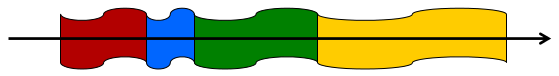
\includegraphics[height=.33in,clip]{xsec-cdf}
	\end{center}
  	\end{figure}

\end{frame}


%%%%%%%%%%%%%%%%%%%%%%%%%%%%%%%%%%%%%%%%%%%%%%%%%%%%%%
%%%%%%%%%%%%%%%%%%%%%%%%%%%%%%%%%%%%%%%%%%%%%%%%%%%%%%
\begin{frame}{Sampling Distance to Collision}

\begin{itemize}
  \item Variable transformation: measure distance in units of mean free path:
  $n = \Sigma(s)s\:,\: dn = \Sigma(s)ds$
  \begin{align*}
    p_c(n)dn &= e^{-n} dn\\
    P_c(n) &= \int_0^n e^{-n'}dn' = -e^{-n'} |_0^n = 1 - e^{-n}
  \end{align*}
  \item Importantly, this is now \underline{independent of the material}
\end{itemize}

\end{frame}


%%%%%%%%%%%%%%%%%%%%%%%%%%%%%%%%%%%%%%%%%%%%%%%%%%%%%%
%%%%%%%%%%%%%%%%%%%%%%%%%%%%%%%%%%%%%%%%%%%%%%%%%%%%%%
\begin{frame}{Cumulative Distribution Functions}

All PDFs, $p(x)$, have an associated \underline{Cumulative Distribution Function (CDF)}, $P(x)$, with the following properties:

\begin{columns}
  \begin{column}{0.5\textwidth}
    \begin{center}
    \textcolor{berkeleygold}{\underline{Continuous}} 
    \end{center}
    %
    \begin{align*}
    P\left\lbrace x' \leq x \right\rbrace &= P(x) = \int_{-\infty}^x p(x')dx'\\
    & \\
    P(-\infty) &= 0 \:,\quad P(\infty) = 1 \\
    0 &\leq P(x) \leq 1 \\
    &\frac{dP(x)}{dx} \geq 0
    \end{align*}
  \end{column}
  \begin{column}{0.5\textwidth}
    \begin{center}
    \textcolor{berkeleyblue}{\underline{Discrete}}  
    \end{center}
    %
    \begin{align*}
    P\left\lbrace x' \leq x \right\rbrace &= P_k \equiv P(x_k) = \sum_{j=1}^k p_j\\
    k &= 1, \dots, N \\
    P_0 &= 0 \:,\quad P_N = 1 \\
    0 &\leq P_k \leq 1 \\
    P_k & \geq P_{k-1} \\
    \end{align*}
  \end{column}
\end{columns}

\end{frame}


%%%%%%%%%%%%%%%%%%%%%%%%%%%%%%%%%%%%%%%%%%%%%%%%%%%%%%
%%%%%%%%%%%%%%%%%%%%%%%%%%%%%%%%%%%%%%%%%%%%%%%%%%%%%%
\begin{frame}{Random Sampling Basics}

  	\begin{figure}
  	\begin{center}
  		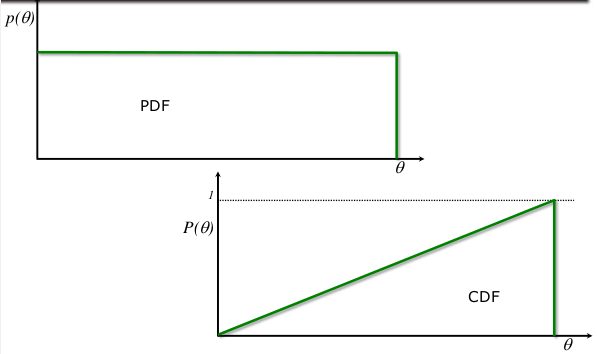
\includegraphics[height=2.75in,clip]{cont-pdf-cdf}
	\end{center}
  	\end{figure}

\end{frame}


%%%%%%%%%%%%%%%%%%%%%%%%%%%%%%%%%%%%%%%%%%%%%%%%%%%%%%
%%%%%%%%%%%%%%%%%%%%%%%%%%%%%%%%%%%%%%%%%%%%%%%%%%%%%%
\begin{frame}{Random Sampling Basics}

  	\begin{figure}
  	\begin{center}
  		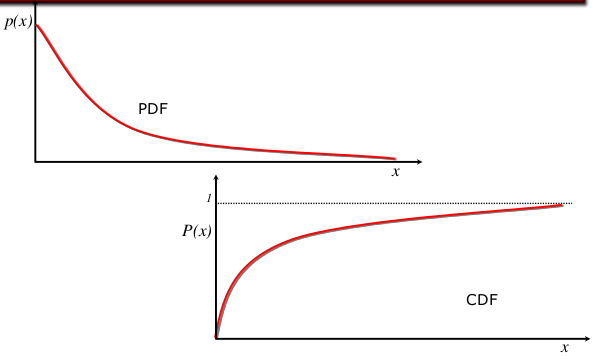
\includegraphics[height=2.75in,clip]{cont-pdf-cdf-2}
	\end{center}
  	\end{figure}

\end{frame}

%%%%%%%%%%%%%%%%%%%%%%%%%%%%%%%%%%%%%%%%%%%%%%%%%%%%%%
%%%%%%%%%%%%%%%%%%%%%%%%%%%%%%%%%%%%%%%%%%%%%%%%%%%%%%
\begin{frame}{Random Sampling Basics}

  	\begin{figure}
  	\begin{center}
  		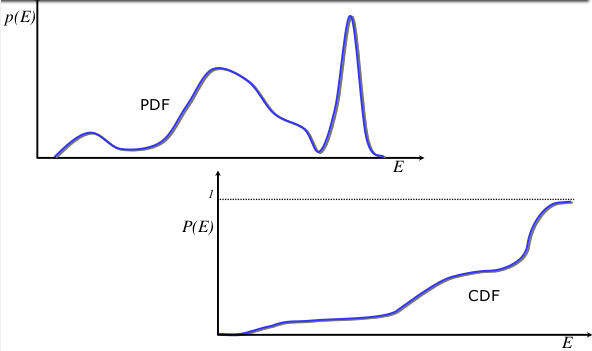
\includegraphics[height=2.75in,clip]{cont-pdf-cdf-3}
	\end{center}
  	\end{figure}

\end{frame}

%%%%%%%%%%%%%%%%%%%%%%%%%%%%%%%%%%%%%%%%%%%%%%%%%%%%%%
%%%%%%%%%%%%%%%%%%%%%%%%%%%%%%%%%%%%%%%%%%%%%%%%%%%%%%
\begin{frame}{Random Sampling Basics}

  	\begin{figure}
  	\begin{center}
  		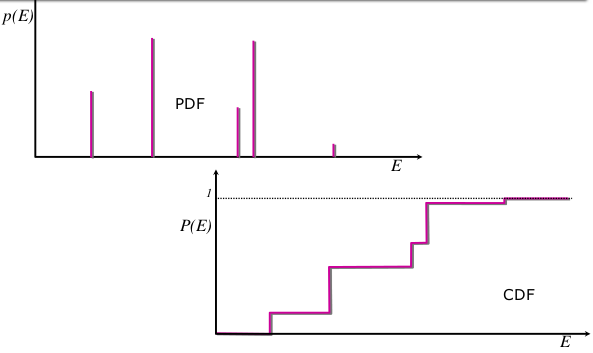
\includegraphics[height=2.75in,clip]{disc-pdf-cdf}
	\end{center}
  	\end{figure}

\end{frame}


%%%%%%%%%%%%%%%%%%%%%%%%%%%%%%%%%%%%%%%%%%%%%%%%%%%%%%
%%%%%%%%%%%%%%%%%%%%%%%%%%%%%%%%%%%%%%%%%%%%%%%%%%%%%%
\begin{frame}{Why Random Sampling}

Various physical phenomena can be
represented by probabilistic distributions

\begin{itemize}
    \item The known probability distribution
represents the \textit{collective} behavior
\vspace*{1em}
    \item We need to know the behavior at \textit{each}
single event
\vspace*{1em}
    \item We need to \underline{recreate} the collective behavior after \underline{many} events
\end{itemize}

\end{frame}


%%%%%%%%%%%%%%%%%%%%%%%%%%%%%%%%%%%%%%%%%%%%%%%%%%%%%%
%%%%%%%%%%%%%%%%%%%%%%%%%%%%%%%%%%%%%%%%%%%%%%%%%%%%%%
\begin{frame}{Random Sampling Purpose}

Use a random process to select a single
value with the following requirements

\begin{itemize}
    \item Each sample should be independent from
other samples
\vspace*{1em}
    \item The PDF formed from a large number of
samples should converge to the initial PDF
\vspace*{1em}
    \item Recover the full resolution of the initial PDF
\end{itemize}

\end{frame}


%%%%%%%%%%%%%%%%%%%%%%%%%%%%%%%%%%%%%%%%%%%%%%%%%%%%%%
%%%%%%%%%%%%%%%%%%%%%%%%%%%%%%%%%%%%%%%%%%%%%%%%%%%%%%
\begin{frame}{Sampling Techniques}

Random sampling uses \underline{uniformly distributed
random variables} to \alert{choose a value for a
variable} according to its probability density
function

    \begin{itemize}
    \item \textit{Basic} sampling techniques
      \begin{itemize}
      \item Direct discrete sampling
      \item Continuous discrete sampling
      \item Rejection sampling
      \end{itemize}
    \pause
    \vspace*{.5em}
    \item \textit{Advanced }sampling techniques
      \begin{itemize}
      \item Histogram
      \item Piecewise linear
      \item Alias sampling
      \item Advanced continuous PDFs
      \end{itemize}
    \end{itemize}

\end{frame}


%%%%%%%%%%%%%%%%%%%%%%%%%%%%%%%%%%%%%%%%%%%%%%%%%%%%%%
%%%%%%%%%%%%%%%%%%%%%%%%%%%%%%%%%%%%%%%%%%%%%%%%%%%%%%
\begin{frame}{Uniformly-Distributed Random Variable}

    \begin{itemize}
    \item Standard notation
      \begin{itemize}
      \item Single random variable: $\xi$
      \item Pair of random variables: $(\xi, \eta)$
      \end{itemize}
    \vspace*{.5em}
    \item PDF for random variables:
    \end{itemize}

\begin{columns}
  \begin{column}{0.5\textwidth}
    %
    \begin{align*}
    p(\xi) = \begin{cases} 
     1 & 0 \leq \xi < 1 \\ 
     0 & \text{ otherwise} 
     \end{cases}
    \end{align*}
  \end{column}
  \begin{column}{0.5\textwidth}
  	\begin{figure}
  	\begin{center}
  		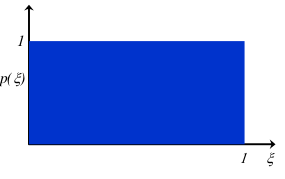
\includegraphics[height=1.5in,clip]{unif-dist-var}
	\end{center}
  	\end{figure}
  \end{column}
\end{columns}

\end{frame}


%%%%%%%%%%%%%%%%%%%%%%%%%%%%%%%%%%%%%%%%%%%%%%%%%%%%%%
%%%%%%%%%%%%%%%%%%%%%%%%%%%%%%%%%%%%%%%%%%%%%%%%%%%%%%
\begin{frame}{Direct Discrete Sampling}

Sampling Procedure

    \begin{itemize}
    \item Generate $\xi$
    \item Determine $k$ such that $P_{k-1} \leq \xi \leq P_k$
    \item Return $x = x_k$
    \end{itemize}

  	\begin{figure}
  	\begin{center}
  		\includegraphics<1>[height=1.5in,clip]{disc-pdf}
  		\includegraphics<2>[height=1.5in,clip]{disc-pdf-samp}
	\end{center}
  	\end{figure}

\end{frame}


%%%%%%%%%%%%%%%%%%%%%%%%%%%%%%%%%%%%%%%%%%%%%%%%%%%%%%
%%%%%%%%%%%%%%%%%%%%%%%%%%%%%%%%%%%%%%%%%%%%%%%%%%%%%%
\begin{frame}{Direct Discrete Sampling}

\vspace*{1 em}
Consider the CDF

  	\begin{figure}
  	\begin{center}
  		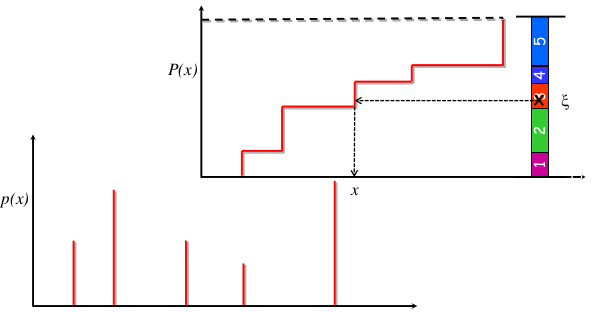
\includegraphics[height=2.5in,clip]{disc-cdf}
	\end{center}
  	\end{figure}

\end{frame}


%%%%%%%%%%%%%%%%%%%%%%%%%%%%%%%%%%%%%%%%%%%%%%%%%%%%%%
%%%%%%%%%%%%%%%%%%%%%%%%%%%%%%%%%%%%%%%%%%%%%%%%%%%%%%
\begin{frame}{Direct Discrete Sampling}

    \begin{itemize}
    \item Requires a table search on $P_k$
      \begin{itemize}
      \item Linear search requires $O(N)$ time
      \item Binary search requires $O(\log_2 N)$ time
      \end{itemize}
    \vspace*{.5em}
    \pause
    \item Special case: Uniform discrete PDF
      \begin{itemize}
      \item $p_k = 1/N$
      \item $P_k = k/N$
      \item $k = \left\lfloor{1 + N\xi}\right\rfloor$ (floor function)
      \end{itemize}
    \end{itemize}

\end{frame}


%%%%%%%%%%%%%%%%%%%%%%%%%%%%%%%%%%%%%%%%%%%%%%%%%%%%%%
%%%%%%%%%%%%%%%%%%%%%%%%%%%%%%%%%%%%%%%%%%%%%%%%%%%%%%
\begin{frame}{Direct Continuous Sampling}

    \begin{itemize}
    \item Can only be used if CDF can be inverted
    \item Direct solution of $P(x)= \xi$
    \item Sampling Procedure:
    \end{itemize}
    \hspace*{3 em} Generate $\xi$ , \hspace*{1 em} Determine $x = P^{-1}(\xi)$
  	\begin{figure}
  	\begin{center}
  		\includegraphics<1>[height=1.5in,clip]{cont-pdf}
  		\includegraphics<2>[height=1.5in,clip]{cont-cdf-on-pdf}
  		\includegraphics<3>[height=1.5in,clip]{cont-cdf-on-pdf-grey}
	\end{center}
  	\end{figure}    
    
\end{frame}


%%%%%%%%%%%%%%%%%%%%%%%%%%%%%%%%%%%%%%%%%%%%%%%%%%%%%%
%%%%%%%%%%%%%%%%%%%%%%%%%%%%%%%%%%%%%%%%%%%%%%%%%%%%%%
\begin{frame}{Direct Continuous Sampling}

    \begin{itemize}
    \item Advantages: 
      \begin{itemize}
      \item Straightforward math \& coding
      \end{itemize}
    \vspace*{1 em}
    \item Disadvantages:
      \begin{itemize}
      \item Can involve computationally slow functions
      \item Not always possible to invert $P(x)$
      \end{itemize}
    \end{itemize}
    
\end{frame}


%%%%%%%%%%%%%%%%%%%%%%%%%%%%%%%%%%%%%%%%%%%%%%%%%%%%%%
%%%%%%%%%%%%%%%%%%%%%%%%%%%%%%%%%%%%%%%%%%%%%%%%%%%%%%
\begin{frame}{Normalization}

    \begin{itemize}
    \item Random sampling depends on \textbf{shape} and not on \sout{magnitude}
    \item Normalization for formal definition of PDF/CDF
required
    \end{itemize}
%
\[
  \begin{aligned}
  \action<+->{f(t)dt &= e^{-\lambda t} dt \:, \quad t > 0 \\}
  %
  \action<+->{F(t) &= \int_{-\infty}^t f(t')dt' = \int_0^t f(t') dt' = \biggl[- \frac{e^{-\lambda t'}}{\lambda} \biggr]_0^t = \frac{1}{\lambda} \bigl(1 - e^{-\lambda t}\bigr)\\
    F(\infty) &= \frac{1}{\lambda}\\}
    %
    \action<+->{\\p(t) &= \lambda f(t) = \lambda e^{-\lambda t} dt \:, \quad t > 0 \\
    %
    P(t) &= \int_{-\infty}^t p(t')dt' = \int_0^t \lambda f(t') dt' = \bigl[e^{-\lambda t'} \bigr]_0^t = 1 - e^{-\lambda t}\\
    %
    P(\infty) &= 1}
  \end{aligned}
\]    
    
\end{frame}


%%%%%%%%%%%%%%%%%%%%%%%%%%%%%%%%%%%%%%%%%%%%%%%%%%%%%%
%%%%%%%%%%%%%%%%%%%%%%%%%%%%%%%%%%%%%%%%%%%%%%%%%%%%%%
\begin{frame}{Shifted Uniform}

\[
  \begin{aligned}
  \action<+->{g(x) dx &= C \quad a \leq x < b\\}
  %
  \action<+->{G(x) &= \int_{-\infty}^x g(x')dx' = C \int_a^x dx' = C\bigl[x' \bigr]_a^x = C \bigl(x - a)\\
    G(\infty) &= G(b) = C(b-a)\\}
    %
    \action<+->{\\p(x) &= \frac{g(x)}{G(\infty)} = \frac{C}{C(b-a)} = \frac{1}{b-a} \quad a \leq x < b\\}
    %
    \action<+->{P(x) &= \int_{-\infty}^x p(x')dx' = \frac{1}{b-a}\int_a^x dx' = \frac{x-a}{b-a}\\
    %
    &\\
    x &= P^{-1}(\xi) = \xi\bigl(b-a\bigr) + a}
  \end{aligned}
\]    
    
\end{frame}


%%%%%%%%%%%%%%%%%%%%%%%%%%%%%%%%%%%%%%%%%%%%%%%%%%%%%%
%%%%%%%%%%%%%%%%%%%%%%%%%%%%%%%%%%%%%%%%%%%%%%%%%%%%%%
\begin{frame}{Simple Line, Slope = $m$}

\[
  \begin{aligned}
  \action<+->{g(x) dx &= mx \qquad 0 \leq x < 1\\}
  %
  \action<+->{G(x) &= \int_{-\infty}^x g(x')dx' = \int_0^x mx' dx' = \frac{m}{2}\bigl[x'^2 \bigr]_0^x = \frac{m}{2} x^2\\q
    G(\infty) &= G(1) = \frac{m}{2}\\}
    %
    \action<+->{\\p(x) &= \frac{mx}{\frac{m}{2}} = 2x \qquad 0 \leq x < 1\\}
    %
    \action<+->{P(x) &= \int_{-\infty}^x p(x')dx' = \int_0^x 2x' dx' = \bigl[x'^2 \bigr]_0^x = x^2\\
    %
    &\\
    x &= P^{-1}(\xi) = \sqrt{\xi} \qquad\text{Independent of }m}
  \end{aligned}
\]    
    
\end{frame}


%%%%%%%%%%%%%%%%%%%%%%%%%%%%%%%%%%%%%%%%%%%%%%%%%%%%%%
%%%%%%%%%%%%%%%%%%%%%%%%%%%%%%%%%%%%%%%%%%%%%%%%%%%%%%
\begin{frame}{Shifted Line}

\[
  \begin{aligned}
  g(x) dx &= m(x - a) \qquad a \leq x < b\\
  %
  G(x) &= \int_{-\infty}^x g(x')dx' = \int_a^x m(x'-a) dx' = \frac{m}{2}\bigl[(x'-a)^2 \bigr]_0^x = \frac{m}{2} (x-a)^2\\
    G(\infty) &= G(1) = \frac{m}{2}(b-a)^2\\
    %
    \\p(x) &= \frac{m(x-a)}{\frac{m}{2}(b-a)^2} = 2 \frac{x-a}{(b-a)^2}\qquad a \leq x < b\\
    %
    P(x) &= \int_{-\infty}^x p(x')dx' = \frac{1}{(b-a)^2}\int_a^x 2(x'-a) dx' = \frac{(x-a)^2}{(b-a)^2}\\
    %
    &\\
    x &= P^{-1}(\xi) = \sqrt{\xi}(b-a) + a \qquad\text{Independent of }m
  \end{aligned}
\]    
    
\end{frame}


%%%%%%%%%%%%%%%%%%%%%%%%%%%%%%%%%%%%%%%%%%%%%%%%%%%%%%
%%%%%%%%%%%%%%%%%%%%%%%%%%%%%%%%%%%%%%%%%%%%%%%%%%%%%%
\begin{frame}{Rejection Sampling}

    \begin{itemize}
    \item Many CDFs cannot be inverted
      \begin{itemize}
      \item e.g.\ Klien-Nishina cross-section
      \end{itemize}
    \vspace*{1 em}
    \pause
    \item Use an approach that is more graphical
      \begin{itemize}
      \item Select a point in a 2-D domain
      \item Determine whether that point is above or below the PDF
      \item Keep those that are below
      \item Start over if above
      \end{itemize}
    \end{itemize}

\end{frame}


%%%%%%%%%%%%%%%%%%%%%%%%%%%%%%%%%%%%%%%%%%%%%%%%%%%%%%
%%%%%%%%%%%%%%%%%%%%%%%%%%%%%%%%%%%%%%%%%%%%%%%%%%%%%%
\begin{frame}{Rejection Sampling}

    \begin{itemize}
    \item Select a bounding function, g(x), such that
      \begin{itemize}
      \item $g(x)= p(x)$ for all $x$
      \item $g(x)$ is easy to sample
      \end{itemize}
    \item Simplest choice is $g(x) = C$
    \item May not be best choice
    \vspace*{1 em}
    \pause
    \item Generate pair of random variables, $(\xi, \eta)$
      \begin{itemize}
      \item $x' = G^{-1} (\xi)$
      \item If $\eta < p(x')/g(x')$, accept $x'$
      \item Else, reject $x'$
      \end{itemize}
    \end{itemize}

\end{frame}

%%%%%%%%%%%%%%%%%%%%%%%%%%%%%%%%%%%%%%%%%%%%%%%%%%%%%%
%%%%%%%%%%%%%%%%%%%%%%%%%%%%%%%%%%%%%%%%%%%%%%%%%%%%%%
\begin{frame}{Rejection Sampling}

  	\begin{figure}
  	\begin{center}
  		\includegraphics<1>[height=2.5in,clip]{rej-samp1}
  		\includegraphics<2>[height=2.5in,clip]{rej-samp2}
  		\includegraphics<3>[height=2.5in,clip]{rej-samp3}
  		\includegraphics<4>[height=2.5in,clip]{rej-samp4}
	\end{center}
  	\end{figure} 

\end{frame}


%%%%%%%%%%%%%%%%%%%%%%%%%%%%%%%%%%%%%%%%%%%%%%%%%%%%%%
%%%%%%%%%%%%%%%%%%%%%%%%%%%%%%%%%%%%%%%%%%%%%%%%%%%%%%
\begin{frame}{Rejection Sampling}

    \begin{itemize}
    \item Advantages
      \begin{itemize}
      \item Computationally simple
      \item Always works
      \end{itemize}
    \vspace*{1 em}
    \pause
    \item Disadvantages
      \begin{itemize}
      \item Will be inefficient if shapes of $g(x)$ and $p(x)$ are not similar
      \end{itemize}
    \end{itemize}
    
    \begin{equation}
    \text{Efficiency }= \frac{\int p(x)dx}{\int g(x) dx} \nonumber
    \end{equation}

\end{frame}


%%%%%%%%%%%%%%%%%%%%%%%%%%%%%%%%%%%%%%%%%%%%%%%%%%%%%%
%%%%%%%%%%%%%%%%%%%%%%%%%%%%%%%%%%%%%%%%%%%%%%%%%%%%%%
\begin{frame}{Random Sampling Summary}

    \begin{itemize}
    \item Physics can be represented \textit{probabilistically}
\pause
\vspace*{.5em}
    \item We can create PDFs and from those generate CDFs
\pause
\vspace*{.5em}
    \item These can be either continuous or discrete
\pause
\vspace*{.5em}
    \item We learned some basic ways to use random numbers to \textit{sample} from these distributions to \alert{simulate physics}
    \end{itemize}
    
\end{frame}


\end{document}
